
\input{../latex_main/main.tex}

%\newcommand{\a}[0]{\mathbf{a}}
%\newcommand{\y}[0]{\mathbf{y}}
\newcommand{\q}[0]{\mathbf{q}}
\newcommand{\Xspace}[0]{\mathcal{X}}

\title[AutoML: Overview]{Multi-criteria Optimization}
\subtitle{Bayesian Optimization}
%TODO: change authors!
\author[Bernd Bischl]{\underline{Bernd Bischl} \and Frank Hutter \and Lars Kotthoff\newline \and Marius Lindauer \and Joaquin Vanschoren}
\institute{}
\date{}



% \AtBeginSection[] % Do nothing for \section*
% {
%   \begin{frame}{Outline}
%     \bigskip
%     \vfill
%     \tableofcontents[currentsection]
%   \end{frame}
% }

\begin{document}

	\maketitle



\begin{frame}[allowframebreaks]{Recap: Bayesian Optimization}

\begin{block}{Advantages of BO}
\begin{itemize}
  \item Sample efficient
  \item Can handle noise
  \item Native incorporation of priors
  \item Does not require gradients
  \item Theoretical guarantees
\end{itemize}
\end{block}

We will now extend BO to multiple cost functions.

\framebreak

\begin{center}
\begin{minipage}{0.75\textwidth}
\begin{algorithm}[H]
    %\DontPrintSemicolon
%    \SetAlgoLined
    \setcounter{AlgoLine}{0}
    \SetKwInOut{Require}{Require}
    \SetKwInOut{Result}{Result}

    \Require{Search space $\pcs$,
    		cost function $\cost$,
    		acquisition function $\acq$, predictive model $\surro$,
    		maximal number of function evaluations $\bobudget$}
    \Result{Best configuration $\finconf$
    (according to $\dataset$ or
    $\surro$)}

	Initialize data $\iter[0]{\dataset}$ with initial observations\;% \leftarrow \varnothing$\;

    \For{$\bocount=1$ \KwTo $\bobudget$}{
		%\While{$B$ not exhausted} {
		Fit predictive model $\iter[\bocount]{\surro}$ on $\iter[\bocount-1]{\dataset}$\;

		Select next query point: $\bonextsample \in \argmax_{\conf \in \pcs} \acq(\conf; \iter[\bocount-1]{\dataset}, \iter[\bocount]{\surro})$\;

		Query $\bonextobs$\;

		Update data: $\iter[\bocount]{\dataset} \leftarrow \iter[\bocount-1]{\dataset} \cup \{\langle \bonextsample, \bonextobs \rangle \}$\;
	}
	\caption*{Bayesian optimization loop}
\end{algorithm}
\end{minipage}
\end{center}
\end{frame}


\begin{frame}{Multi-Criteria Bayesian Optimization}

\textbf{Goal}: Extend Bayesian optimization to multiple cost functions

$$
\min_{\conf \in \pcs}  \cost(\conf) \Leftrightarrow \min_{\conf \in \pcs} \left(\cost_1(\conf), \cost_2(\conf), ..., \cost_m(\conf)\right).
$$


    \vspace{0.5cm}

There are two basic approaches:

\begin{enumerate}
        \item Simplify the problem by scalarizing the cost functions, or
        \item define acquisition functions for multiple cost functions.
\end{enumerate}

\end{frame}

\begin{frame}{Scalarization}

    \textbf{Idea:} Aggregate all cost functions


    $$\min_{\conf \in \pcs} \sum_{i = 1}^m w_i \cost_i(\conf) \qquad \text{with} \quad w_i \ge 0 $$

    \begin{itemize}
        \item \textbf{Obvious problem:} How to choose $w_1, \dots, w_m$?
            \begin{itemize}
                \item Expert knowledge?
                \item Systematic variation?
                \item Random variation?
            \end{itemize}
        \item If expert knowledge is not available a-priori, we need to ensure that different trade-offs between cost functions are explored.
            \item Simplifies multi-criteria optimization problem to single-objective \\$\longrightarrow$ Bayesian optimization can be used without adaption of the general algorithm.
    \end{itemize}

\end{frame}

\begin{frame}{Scalarization: ParEGO~\litw{\href{https://www.cs.bham.ac.uk/~jdk/parego/ParEGO-TR3.pdf}{Knowles. 2006}}}

    Scalarize the cost functions using the augmented Tchebycheff norm / achievement function

    $$
    c = \max_{i=1,\dots,m}\left(w_i \cost_i(\conf)\right) + \rho \sum_{i=1}^m w_i\cost_i(\conf),
    $$

    \begin{itemize}
        \item The weights $w \in W$ are drawn from
            $$
                W = \left\{ w = (w_1, \dots, w_m) | \sum_{i=1}^m w_i = 1, w_i = \frac{l}{s} \wedge, l \in 0,\dots,s\right\},
            $$
            with $|W| = {{s+m-1}\choose{k-1}}1$.
        \item New weights are drawn in every BO iteration.
        \item $\rho$ is a small parameter suggested to be set to $0.05$.
        \item $s$ selects the number of different weights to draw from.
    \end{itemize}

\end{frame}

\begin{frame}{Why the Tchebycheff norm?}

    \begin{center}
        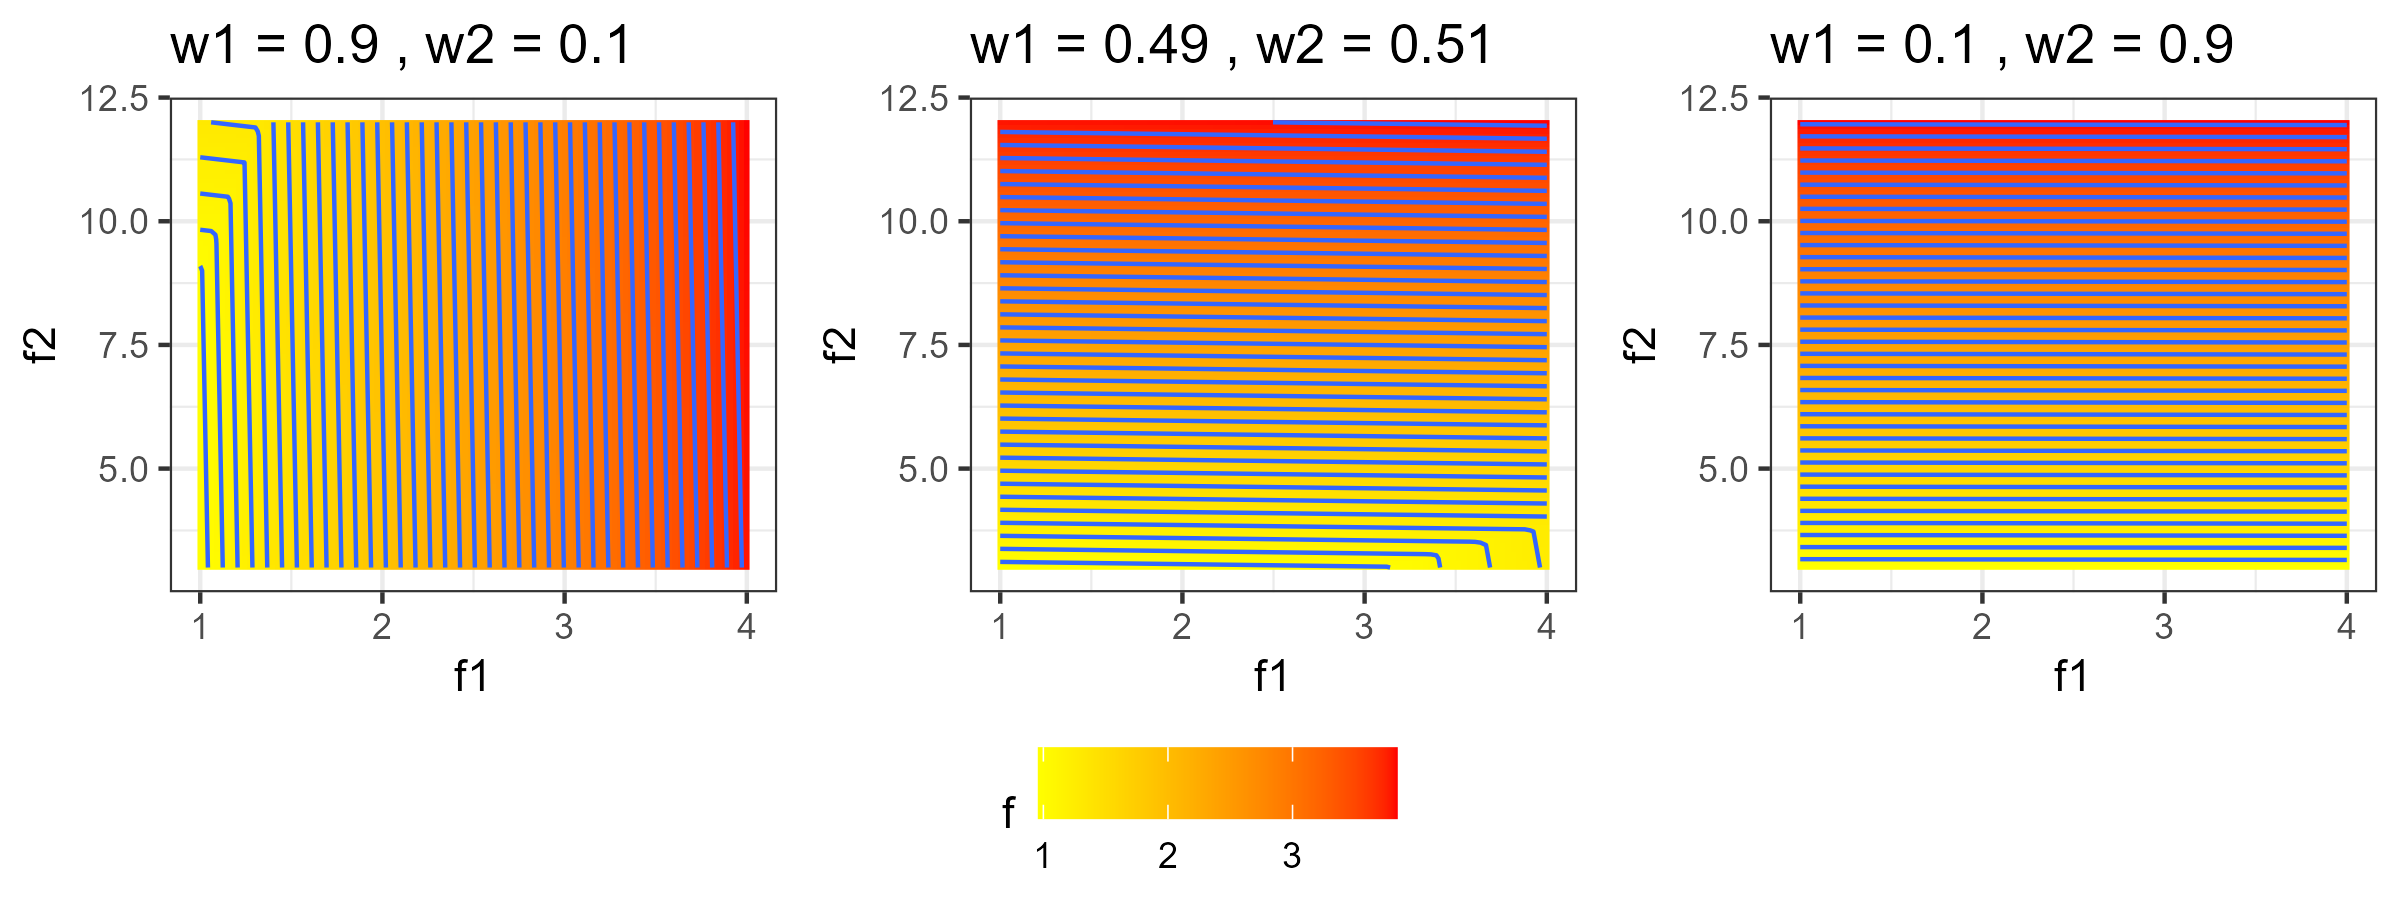
\includegraphics[scale=0.08]{images/parego_viz}
    \end{center}
        %Example of 3 different ParEGO scalarizations of the two objective functions $\cost_1(\conf) = (\conf - 1)^2$ and $c_2(\conf) = 3(\conf - 2)^2$.
    $$
    c = \max_{i=1,\dots,m}\left(w_i \cost_i(\conf)\right) + \rho \sum_{i=1}^m w_i\cost_i(\conf),
    $$
    \begin{scriptsize}
    \begin{itemize}
        \item The norm consists of two components:
            \begin{itemize}
                    \item $\max_{i=1,\dots,m}\left(w_i \cost_i(\conf)\right)$ takes only the maximum weighted cost into account.
                    \item $\sum_{i=1}^m w_i\cost_i(\conf)$ is the weighted sum of all cost functions.
            \end{itemize}
        \item $\rho$ describes the trade-off between these components.
        \item By the randomized weights in each iteration and the usually small value of $\rho = 0.05$, this allows exploration of extreme points of single cost functions.
        \item One can prove: \textbf{Every solution of the scalarized problem is pareto-optimal!}
    \end{itemize}
    \end{scriptsize}
\end{frame}

\begin{frame}{ParEGO Algorithm}


\begin{center}
\begin{minipage}{0.8\textwidth}
\begin{algorithm}[H]
    %\DontPrintSemicolon
%    \SetAlgoLined
    \setcounter{AlgoLine}{0}
    \SetKwInOut{Require}{Require}
    \SetKwInOut{Result}{Result}

    \Require{Search space $\pcs$,
    		cost function $\cost$,
    		acquisition function $\acq$, predictive model $\surro$,
            maximal number of function evaluations $\bobudget$, $\rho$, $l$, $s$}
    \Result{Best configuration $\finconf$
    (according to $\dataset$ or
    $\surro$)}

	Initialize data $\iter[0]{\dataset}$ with initial observations\;% \leftarrow \varnothing$\;

    \For{$\bocount=1$ \KwTo $\bobudget$}{
		%\While{$B$ not exhausted} {
        Sample $w$ from  $\left\{ w = (w_1, \dots, w_m) | \sum_{i=1}^m w_i = 1, w_i = \frac{l}{s} \wedge, l \in 0,\dots,s\right\}$;

        Compute scalarization $c^{(t)} = \max_{i=1,\dots,m}\left(w_i \cost_i(\conf)\right) + \rho \sum_{i=1}^m w_i\cost_i(\conf)$;

		Fit predictive model $\iter[\bocount]{\surro}$ on $\iter[\bocount-1]{\dataset}$\;

		Select next query point: $\bonextsample \in \argmax_{\conf \in \pcs} \acq(\conf; \iter[\bocount-1]{\dataset}, \iter[\bocount]{\surro})$\;

		Query $\bonextobs$\;

		Update data: $\iter[\bocount]{\dataset} \leftarrow \iter[\bocount-1]{\dataset} \cup \{\langle \bonextsample, \bonextobs \rangle \}$\;
	}
	\caption*{ParEGO loop}
\end{algorithm}
\end{minipage}
\end{center}
\end{frame}


%\begin{frame}{ParEGO Example}

%    \begin{center}
%        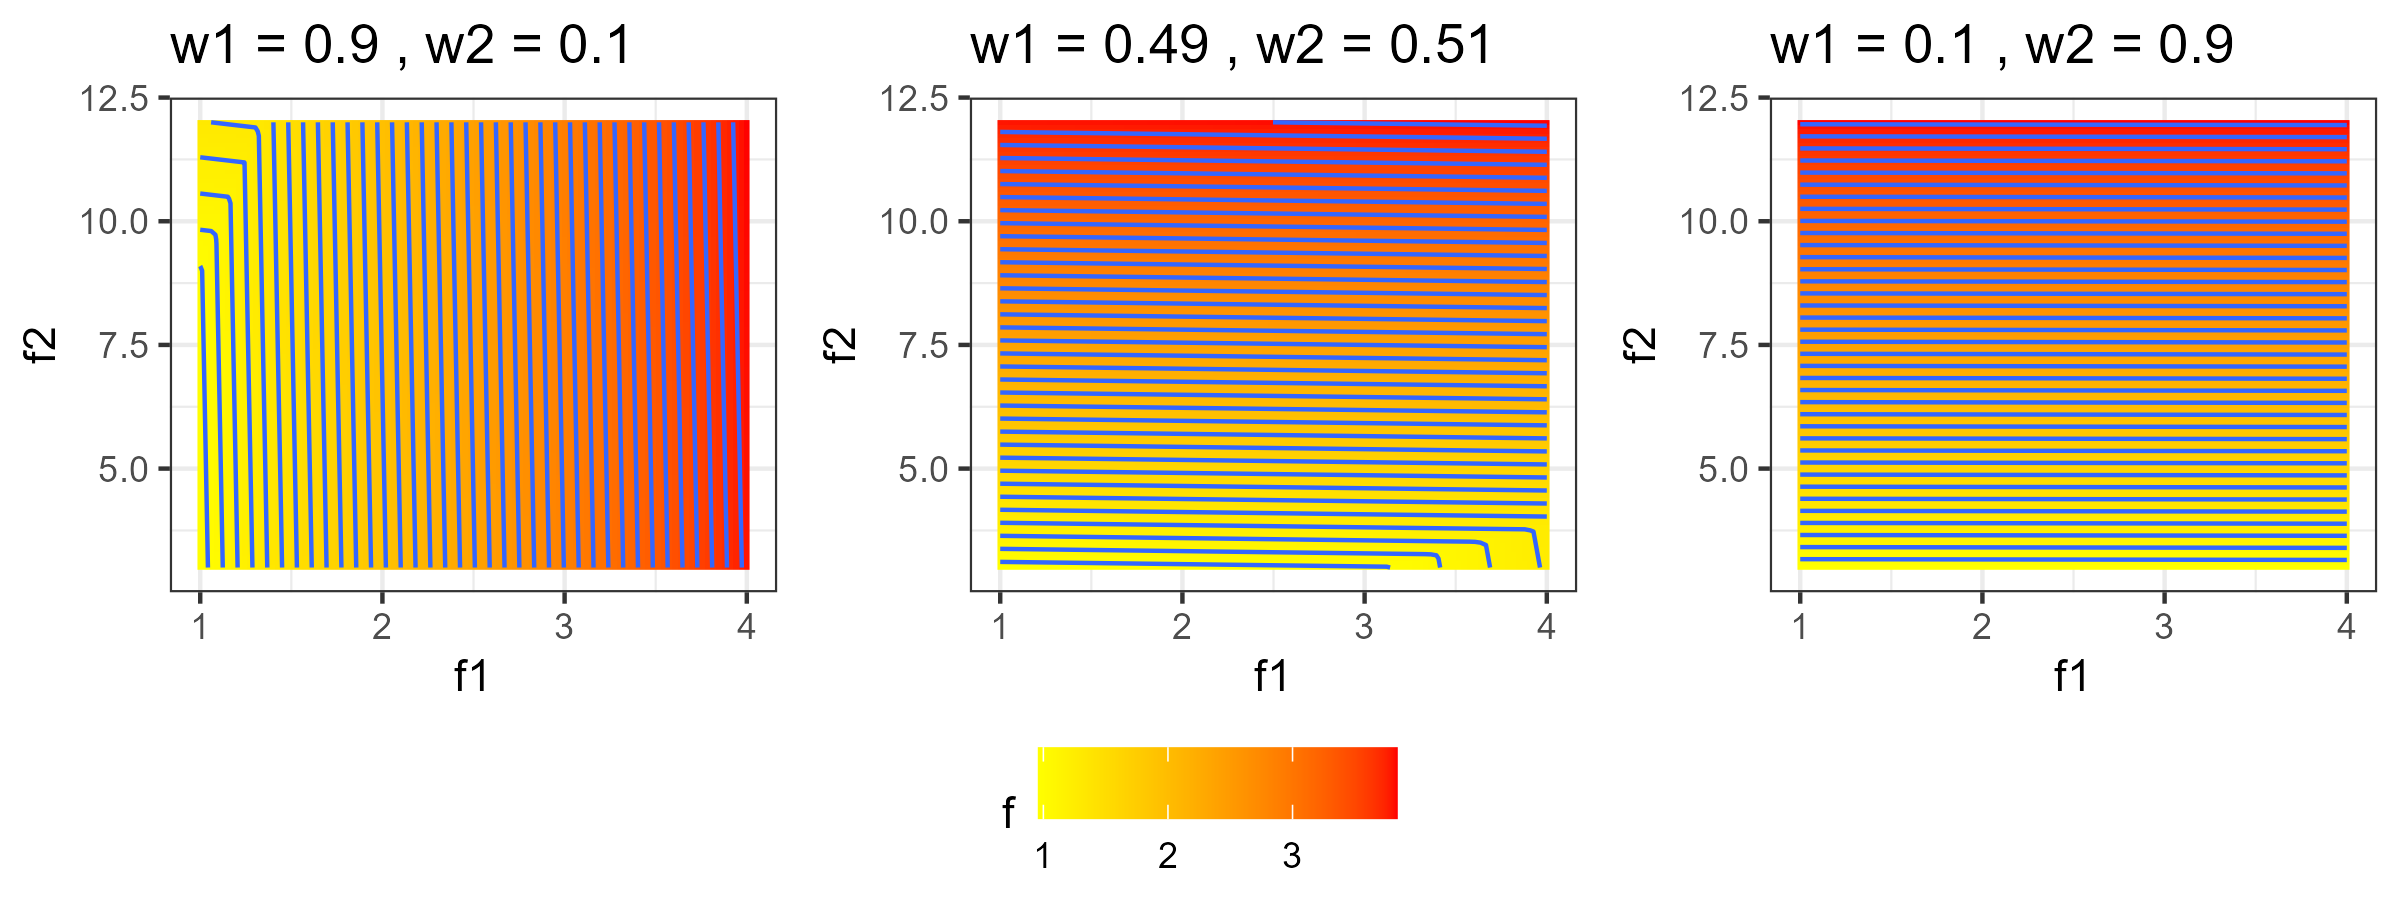
\includegraphics[scale=0.15]{images/parego_viz}
%    \end{center}
%        Example of 3 different ParEGO scalarizations of the two objective functions $\cost_1(\conf) = (\conf - 1)^2$ and $c_2(\conf) = 3(\conf - 2)^2$.
%\end{frame}


\begin{frame}{Hypervolume based Acquisition Functions}

    \textbf{Idea:} Define acquisition function that directly models contribution to dominated HV.

            $$
            \max(0, S(\mathcal{P} \cup \conf, R) - S(\mathcal{P}, R))
            $$
    \begin{center}
        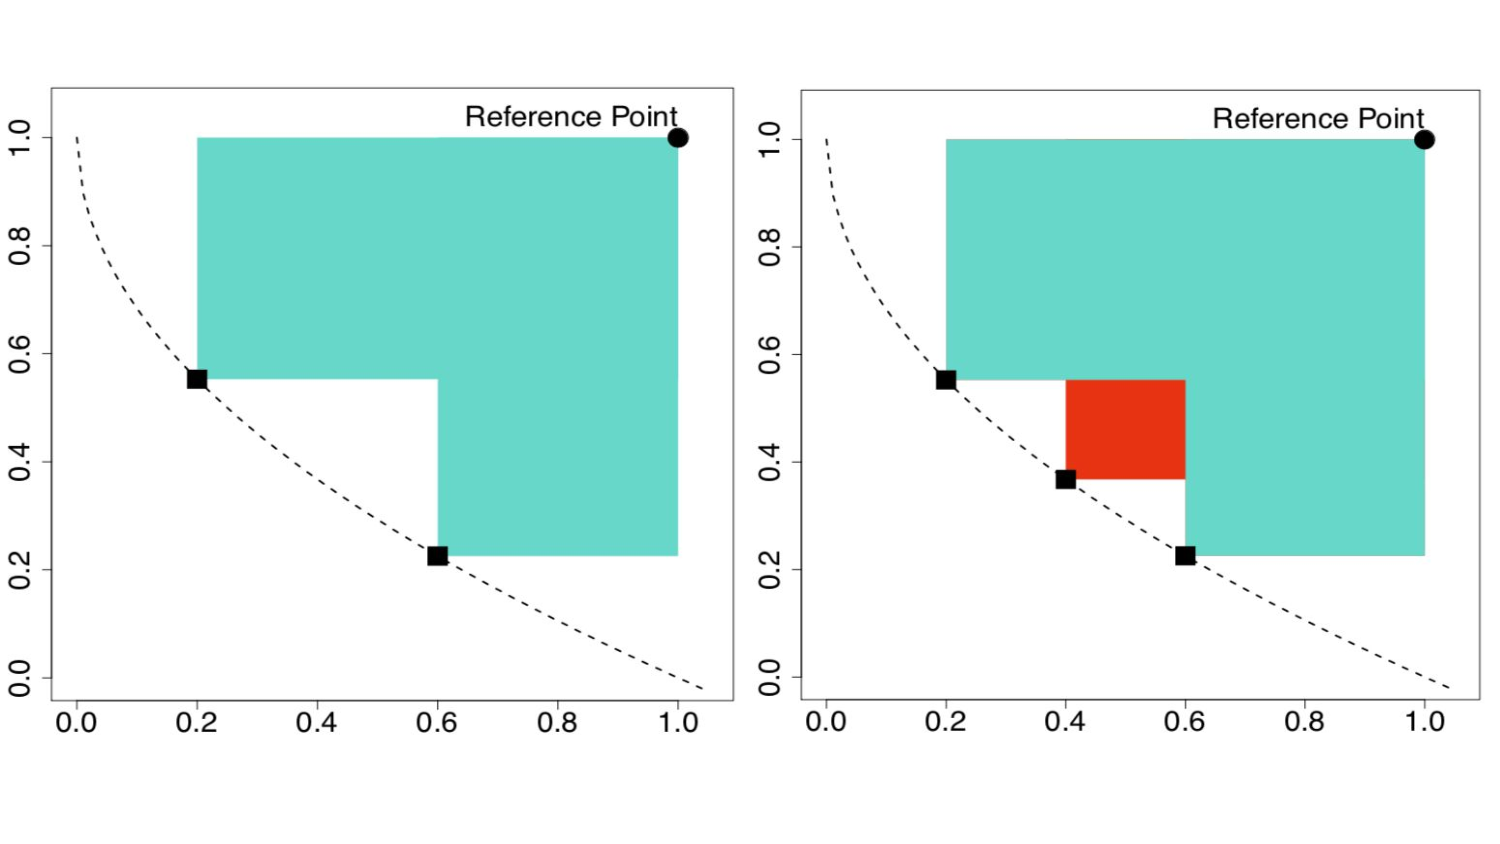
\includegraphics[scale=0.22]{images/hv_contribution}
    \end{center}

    \begin{itemize}
            \item Fit $m$ single-objective surrogate models $\surro_1, \dots, \surro_m$
            \item Acquisition function takes all surrogate models into account.
            \item Single-criteria optimization of acquisition function.
    \end{itemize}

\end{frame}

\begin{frame}[allowframebreaks]{S-Metric Selection-based EGO}

    Using the Lower Confidence bound $u_{\text{LCB}, 1}(\conf), \dots, u_{\text{LCB}, m}(\conf)$, an optimistic estimate of hypervolume contribution can be calculated.

    \begin{center}
        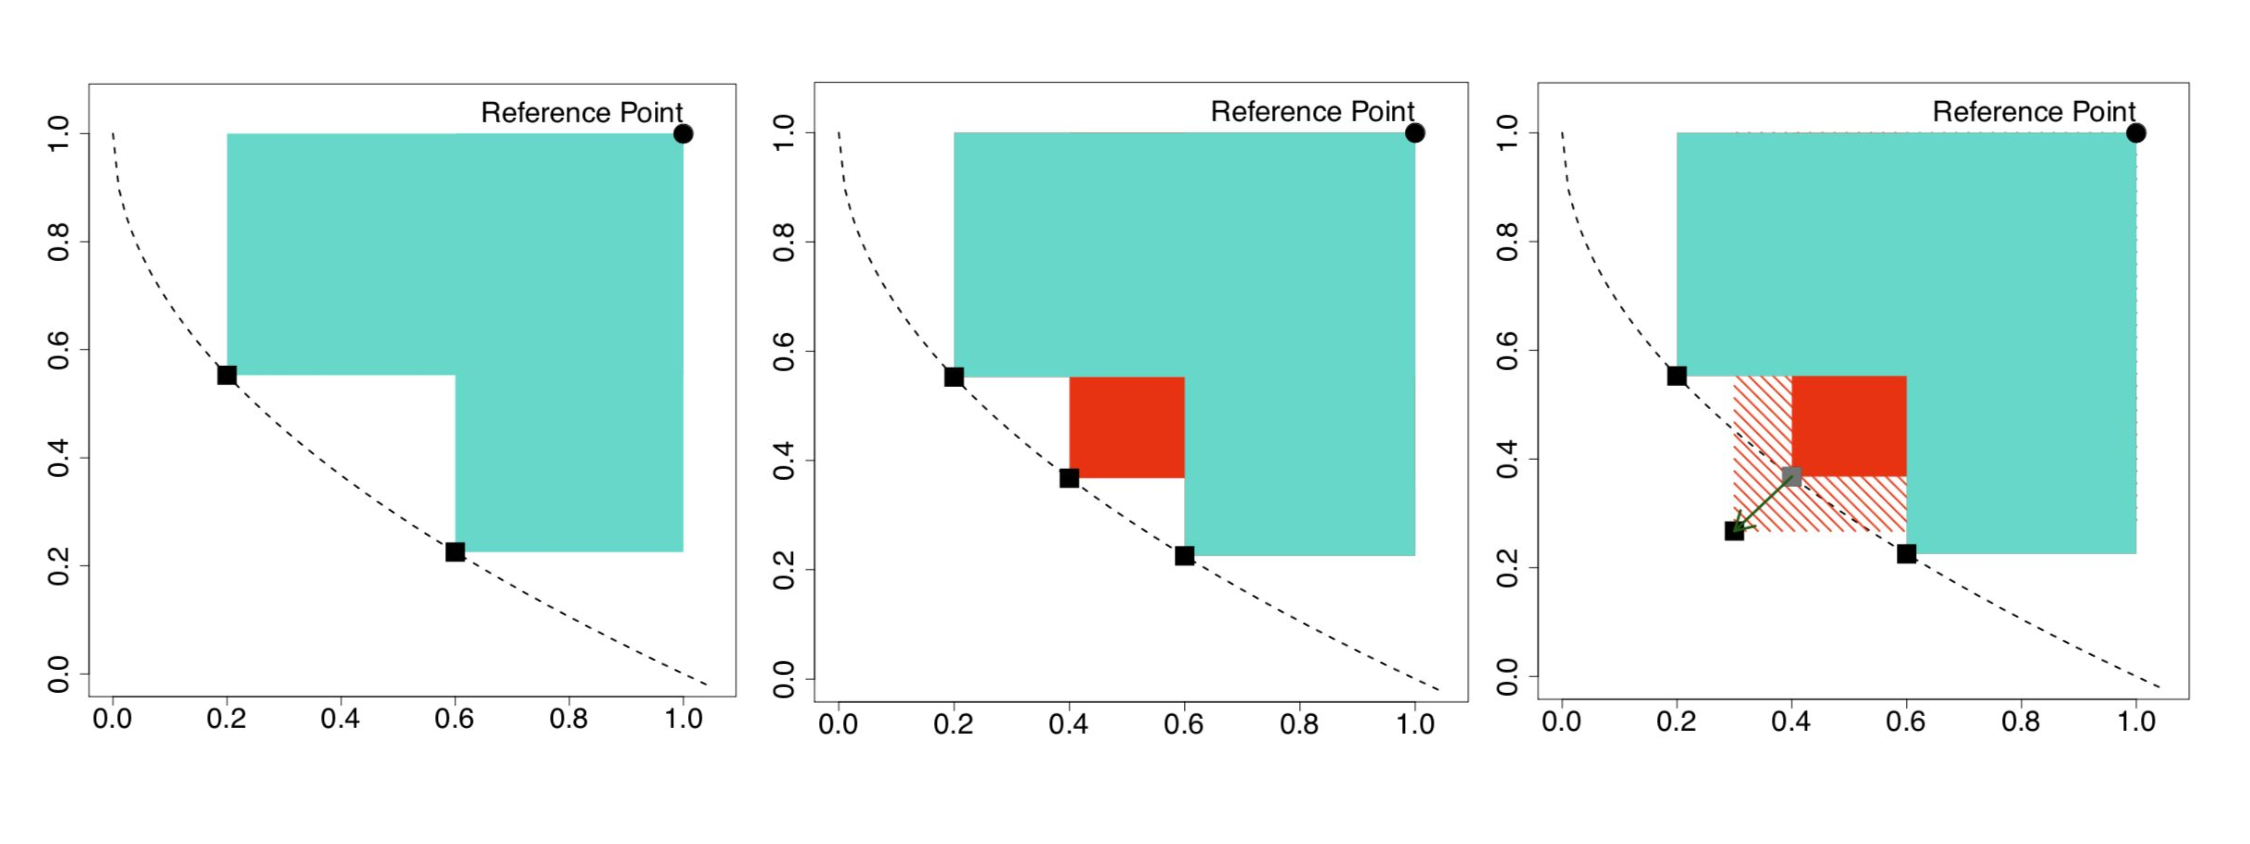
\includegraphics[scale=0.35]{images/hv_contribution_2}
    \end{center}

    \framebreak

    \textbf{Problem}: Based on the way the hypervolume contribution is measured large plateaus of zero improvement are present.
    \begin{itemize}
        \item These make optimization much harder.
         \item An adaptive penalty is added to regions in which the lower confidence bound is dominated.
    \end{itemize}

    \vspace{0.5cm}

        This method is referred to as SMS-EGO~\lit{\href{https://doi.org/10.1007/978-3-540-87700-4_78}{Ponweiser et al. 2008}}.
\end{frame}

\begin{frame}{Further Hypervolume based Acquisition Functions}

    \textbf{Expected Hypervolume Improvement (EHI)}~\lit{\href{https://doi.org/10.1016/j.swevo.2018.10.007}{Yang et al. 2019}}

$$
    u_{EI, \mathcal{H}}(\conf) = \int_{-\infty}^{\infty} p(\cost \mid \conf) \times \mathcal{H}(\conf)\;\; d\cost,\
$$
    with $\mathcal{H}(\conf) = S(\mathcal{P} \cup \conf, R) - S(\mathcal{P}, R))$.

    \begin{itemize}
        \item Direct extension of $u_{EI}$ to the hypervolume.
        \item $p(\cost \mid \conf)$ is the joint density of the surrogate model predictions at $\conf$.
        \item As the surrogates are GPs and modeled independently of each other, this is just an integral over $m$ univariate normal distributions.
        \item Efficient computations for $m \le 3$ exist, beyond that expensive simulation-based computation is required.
    \end{itemize}


    \vspace{0.5cm}
Further hypervolume based acquisition functions:

    \begin{itemize}
        \item \textbf{Stepwise Uncertainty Reduction} (SUR) based on the probability of improvement.
        \item \textbf{Expected Maximin Improvement} (EMI) based on the $\epsilon$-indicator.
    \end{itemize}


\end{frame}

\begin{frame}{Hypervolume based BO Algorithm}


\begin{center}
\begin{minipage}{0.8\textwidth}
\begin{algorithm}[H]
    %\DontPrintSemicolon
%    \SetAlgoLined
    \setcounter{AlgoLine}{0}
    \SetKwInOut{Require}{Require}
    \SetKwInOut{Result}{Result}

    \Require{Search space $\pcs$,
    		cost function $\cost$,
    		acquisition function $\acq$, predictive model $\surro$,
            maximal number of function evaluations $\bobudget$}
    \Result{Best configuration $\finconf$
    (according to $\dataset$ or
    $\surro$)}

	Initialize data $\iter[0]{\dataset}$ with initial observations\;% \leftarrow \varnothing$\;

    \For{$\bocount=1$ \KwTo $\bobudget$}{
		%\While{$B$ not exhausted} {

		Fit predictive models $\iter[\bocount]{\surro_1}, \dots, \iter[\bocount]{\surro_m}$ on $\iter[\bocount-1]{\dataset}$\;

		Select next query point: $\bonextsample \in \argmax_{\conf \in \pcs} \acq(\conf; \iter[\bocount-1]{\dataset}, \iter[\bocount]{\surro_1}, \dots, \iter[\bocount]{\surro_m}))$\;

		Query $\bonextobs$\;

		Update data: $\iter[\bocount]{\dataset} \leftarrow \iter[\bocount-1]{\dataset} \cup \{\langle \bonextsample, \bonextobs \rangle \}$\;
	}
	\caption*{Hypervolume based Bayesian optimization loop}
\end{algorithm}
\end{minipage}
\end{center}
\end{frame}

% NOTE: We decided to scrap mspot
% \begin{frame}{Multi-Criteria Optimization of Acquisition Functions}
%     \textbf{Goal:} Apply multi-criteria optimization methods on acquisition to approximate a pareto front.

%     \begin{itemize}
%        \item Separate surrogate model $\surro_1, \dots, \surro_m$ for each cost function.
%        \item Apply Multi-Criteria optimization (e.g. NSGA-II) to approximate pareto front over acquisition functions.
%        \item Select a single configuration from the estimated pareto front, e.g., by hypervolume contribution.
%     \end{itemize}
% \end{frame}


\end{document}
